%!TEX root = ../main.tex
Nowadays, solving hard combinatorial optimization problems is a very important field of artificial intelligence. Different techniques using heuristics and metaheuristics are used to solve these problems. Ant Colony Optimization (ACO) is one of these metaheuristics approaches that appeared in 1999 \cite{dorigo1999ant} \cite{corne1999ant}. This metaheuristic has proven to be very effective in various fields of applications such as in vehicle routing problems. Solving a problem using an ACO metaheuristic requires a lot of programming work as there is no ACO solver at the moment. One inconvenient with ACO is the complex mapping of a problem into something that can be used by this metaheuristic to build solutions. It is difficult to adapt an application of ACO from one problem to another. When using ACO, each constraint added or removed in a problem changes the whole implementation. 

The goal of this master thesis is to create a framework that allows a user to use ACO to solve different routing problems by adding its own constraints in an easy way and to give a fixed representation of these constraints.

\section{Ant Colony Optimization}\label{whatisACO}
The family of Ant Colony Optimization metaheuristic is originated in the observation of the behaviour of real ants and their interactions with their environment. These observations have lead to the creation of a metaheuristic now widely used.

\subsection{Biological inspiration}\label{bio}
The original idea comes from the observation of the exploitation of the food resources by the ants. Although ants have limited cognitive resources as individuals, when working together they are able to find the shortest route from their nest to a food source.
Biologists made a series of experiments: An ant colony has the choice between two paths of unequal length that lead to a food source. After some time, they eventually use the shortest path.
The biologists explain this behavior in the following way:
\begin{enumerate}
	\item An ant (called scout) walks randomly around the colony.
	\item If that ant discovers a food source, she comes back to the nest, leaving a trail of pheromones; see figure \ref{choice} (a).
	\item These pheromones being attractive for the other ants, the other ants will have a tendency to follow the pheromone trail; see figure \ref{choice} (b).
	\item Coming back to the nest, these new ants will reenforce the trail.
	\item If two paths are available to reach the same food source, the shortest one will be, in a fixed time interval, used by more ants than the longest one because of the evaporation.
	\item The shortest path will be more and more attractive to the ants.
	\item The longest path will eventually disappear, pheromones being volatile; see figure \ref{choice} (c). 
\end{enumerate}
 
\begin{figure}
	\centering
		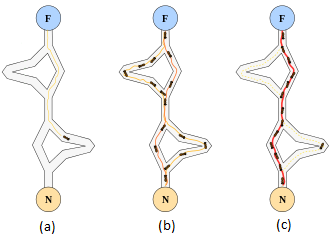
\includegraphics{images/330px-Aco_branches.png}
	\caption{Food discovery by an ant colony}
	\label{choice}
\end{figure}

The ants use the environment as a communication support. They exchange information by dropping pheromones on their lines of movement. The information has a local impact: only an ant that is close to the pheromones can access them and use them. The French entomologist Pierre-Paul Grasse created the word \textit{"stigmergy"} to describe this type of communication where the actual exploration is stimulated by the performance already achieved \cite{dorigo2006ant}. 
This mechanism permits to an ant colony to solve a problem that is too complex for one single ant. It is a good example of a self-organized system. This system relies on positive feedback (the pheromone trail attracts other ants that reenforce the trail) and negative feedback (dissipation of the pheromones by evaporation over time).
Theoretically, if the amount of pheromone on a path is constant over time (there is no evaporation), no path would be chosen, but the positive and negative feedback permits the amplification of the pheromone trail on a particular path and not the other. This leads to the choice of this path.

\subsection{The Ant Colony Optimization Metaheuristic}\label{metaheuristic}

\subsubsection{History}
After the elaboration of the stigmergy theory by Pierre-Paul Grasse in 1959, many researchers and academic experts have analyzed ants and how they behave. In 1989, the works of Goss, Aron, Deneubourg and Pasteels on the collective behavior of the argentine ants provided the necessary ground work for the development of ant colony algorithms. In 1992, Marco Dorigo proposed the Ant System in his doctoral thesis \cite{dorigo1991ant}. This was the first algorithm based on ant behavior. The Ant System will be improved in several ways to become in 1997 the Ant Colony System. The term Ant Colony Optimization metaheuristic (ACO) appears in 1999 to regroup the algorithms that builds solutions using the Ant (Colony) System. Until now, ACO has evolved in different ways and has been applied to a lot of different problems (see section \ref{existing}).

\subsubsection{Optimization problem}
An optimization problem, in mathematics and computer sciences, is the problem of finding the best solution to a problem, using a given quantitative criterion, from the set of all feasible solutions. There are two categories of optimization problem depending on whether the variables are continuous or discrete. If the variables are discrete, the problem is called a combinatorial optimization problem. The solution to that type of problem is in the form of an integer, a permutation or a graph from a finite set. Some of these problems are known as NP-hard. To solve these NP-hard problems, heuristics and metaheuristics are used. These techniques aim to solve these optimization problems.

\subsubsection{Metaheuristic}
A metaheuristic is an optimization algorithm aiming at the solving of an optimization problem. Metaheuristic are usually iterative stochastic algorithms progressing through a global optimum. They behave like search algorithms, trying to learn some characteristics of a problem to find an approximation of the best solution.
Metaheuristics use their history to guide the optimization on the following iterations. In the simplest case, they use only one previous state to determine the next iteration. We speak in that case of a method without memory. However, a lot of metaheuristics use a more evolved memory on short term or long term, using a set of parameters describing the research.
The use of metaheuristics has significantly increased the ability of finding very high-quality solutions to hard, practically relevant combinatorial optimization problems in a reasonable time. \cite{dorigo2004ant}



\subsubsection{Ant Colony Optimization}
Ant colony optimization is a metaheuristic in which a colony of artificial ants cooperates in finding good solutions to difficult discrete optimization problems \cite{dorigo2004ant}. In this metaheuristic, we let simple agents (ants) build good solutions using their own channel of communication that is the pheromone trail. This type of communication permits to learn from the previous solutions constructed by the ants.

In ACO, an artificial ant is a constructive procedure that builds a solution incrementally. ACO can therefore be used in any problem where a constructive heuristic can be defined.

The ants in ACO implement a randomized construction heuristic that builds a solution by iteratively adding components to partial solutions by taking into account in a probabilistic way:
\begin{itemize}
	\item heuristic information about the problem instance being solved.
	\item pheromone trails which change dynamically at run-time and reflect the ants search experience.
\end{itemize}


\subsubsection{Problem Representation}
Consider the static (non time-dependent) minimization problem $(S,f,\Omega)$ where $S$ is the set of candidate solutions, $f$ is the objective function that assigns a cost $f(s)$ to each candidate solution $s \in S$ and $\Omega$ is a set of constraints.
The goal is to find an optimal feasible solution $s^*$ : A minimum cost feasible solution to the problem.

This problem can be mapped in a way that will be usable by the ants. The mapping of the problem is characterized by the following items\cite{dorigo2004ant}:
\begin{itemize}
	\item A finite set $C = {c_1,c_2,...,c_{N_C}}$ of components is given, $N_C$ is the number of components. Each $c_i$ are components of the set of candidate solutions.
	\item The states of the problem are defined in terms of sequences $x = [c_i, c_j, ...,c_h,...]$ of finite length over the elements of C. The set of all possible states is denoted by $X$. The maximum length of a sequence $x$ is bounded.
	\item The set of possible solutions is denoted by $S$. $S \subseteq X$.
	\item The set of feasible solutions is denoted by $\tilde{S}$. $\tilde{S} \subseteq S$. This set of feasible solutions is obtained from $S$ via the constraints $\Omega$.
	\item A non-empty set of optimal solutions $S^* \subseteq S$.
	\item A cost $g(s,t)$ is associated with each solution $s \in S$. In most case $g(s) \equiv f(s)$
	\item Sometimes a cost can be associated with states other than candidate solutions.
\end{itemize}

With this formulation, an ant can build a solution by performing a randomized path on the completely connected graph $G_C = (C,L)$ The nodes of the graph are the components $C$ described above and the set of arcs $L$ fully connects the components of C. The constraints $\Omega$ are implemented in the policy followed by the ants. This permits to chose if the constraints must be implemented in a hard way (the ants can not build infeasible solutions - solutions that violate constraints) or in a soft one (the ants are allowed to build infeasible solutions that will be penalized as a function of their degree of infeasibility).

\section{State of the Art}\label{state}
\subsection{Existing applications of ACO algorithms}\label{existing}
ACO algorithms have been applied to different types of problems and have been widely studied. Table \ref{tab:existing} provides a quick summary of the current applications of ACO algorithms. 

\begin{table}
\centering
\begin{tabular}{|l|l|}
	\hline
	Problem type & Problem name\\
	\hline
	Routing & Traveling salseman \\
	&Vehicle routing \\
	&Sequential ordering \\[6pt]
	Assignment & Quadratic assignment \\
	&Graph coloring\\
	&Generalized assignment\\
	&Frequency assignment\\
	&University course timetabling\\[6pt]
	Scheduling & Job shop\\
	&Open shop\\
	&Flow shop \\
	&Total tardiness\\
	&Total weighted tardiness\\
	&Project sheduling\\
	&Group shop\\[6pt]
	Subset & Multiple knapsack\\
	&Max independent set\\
	&Redundancy allocation\\
	&Set covering\\
	&Weight constrained graph tree partition\\
	&Arc-weighted l-cardinality tree\\
	&Maximum clique\\[6pt]
	Network routing& Connection-oriented network routing\\
	&Connectionless network routing\\
	&Optical network routing\\
	\hline
\end{tabular}
\caption{Existing applications of ACO algorithms}
\label{tab:existing}
\end{table}

In this thesis we will focus on the traveling salesman problem, the capacitated vehicle routing problem and the vehicle routing problem with time windows. These three will be explained in more detail in section \ref{poi}.

\subsection{Results and usage of these applications}\label{results}
ACO algorithms have for the moment comparable performances to the best existing methods to solve some of the problems listed here after : the sequential ordering problem \cite{gambardella2000ant}, the vehicle routing with time window problem \cite{gambardella1999macs}, the quadratic assignment problem \cite{stutzle2000max}, the group shop scheduling problem \cite{blum2002aco}, the arc-weighted l-cardinality tree problem \cite{blum2005new}, the shortest common supersequence problem \cite{michel1999aco} and finally network routing problems \cite{varela1999ant}. The success of these algorithms attracted widespread attention throughout the scientific community. This encouraged research in the field of ACO applications.

 
\section{Problems of Interest}\label{poi}
This thesis focuses on three problems: the Traveling Salesman problem, the capacitated vehicle routing problem and the vehicle routing problem with time windows. These problems are described hereafter. 

\subsection{Traveling Salesman Problem}
The traveling salesman problem is a mathematical problem where, given a set of cities for which the distance between each of them is known, the goal is to find the shortest path that passes through all of these cities exactly once. It's an optimization problem for which there is no known polynomial time algorithm. The decisional version ( for a distance $D$, is there a path that passes through all the cities with a length less or equal to $D$? ) is known as an NP-Hard problem.
More formally, the TSP can be represented as a complete weighted graph $ G = (N,A) $, $N$ being the set of nodes representing the cities, and $A$ the set of arcs. Each arc $(i,j) \in A$ is assigned a value $d_{ij}$ (the distance between the two cities $i$ and $j$ ($i,j \in N$)). We will work only with symmetric TSP so $d_{ij} = d_{ji}$ for all vertices. The goal is to find the minimum length Hamiltonian cycle of this graph $G$. An Hamiltonian cycle is a closed path that visits each nodes $n \in N$ of $G$ exactly once. An optimal solution to this problem is thus a permutation $\pi$ of the node index such that the length $f(\pi)$ is minimal. $\pi$ is thus a bijection on the set of nodes $N$ on itself. $\pi (i)$ denotes the $i^{th}$ element of the permutation $\pi$. $f(\pi)$ is given by \cite{dorigo2004ant} : 

\begin{equation}
f(\pi) = \sum_{i=1}^{n} d_{\pi(i)\pi(i+1)} + d_{\pi(n)\pi(1)}
\label{eq:distance}
\end{equation}

In equation \ref{eq:distance}, a sum of the distance between all consecutive node in permutation $\pi$ is made. To that sum, is added the distance between the first and the last node of the permutation to close the cycle. This gives the value to the length of the permutation $\pi$.


\subsection{Vehicle Routing Problem}
The vehicle routing problem (VRP) is a combinatorial optimization problem. The goal is to serve a number of customers with a fleet of vehicles. It is an important problem in the field of transportation, distribution and logistics.
The distribution of goods concerns the service of a set of customers by a set of vehicles which are located in one or more depots. In this thesis, we only work with one depot. A solution of a VRP consists in the determination of a set of routes, each traveled by a single vehicle that starts and ends at the depot, such that all the needs of the customers are fulfilled and no operational constraints are violated (maximal load of a truck for example).
In this thesis, we work with the capacitated Vehicle Routing Problem and with the Vehicle Routing Problem with Time-Windows. This is why we develop these two more in detail.

\subsubsection{Capacitated Vehicle Routing Problem}
In the CVRP, the customers correspond to delivery points and the demands of these customers are known in advance. The vehicles of the fleet are all the same and are based in a single central depot. In this problem, the only restriction is the capacity of the vehicles. The goal is to minimize the total cost to serve all of the customers (the travel time, the number of routes, or the length of the route).
Here is the mathematical description of the problem: 
As for the TSP, the problem is represented with a complete graph $G=(N,A)$ where $N = {0,...,n}$ is the node set and $A$ is the arc set. The depot corresponds to the node $0$. The nodes $1,...,n$ correspond to the customers.
Again, with each arc $(i,j) \in A$ is associated a cost $d_{ij}$ that represents the cost to travel from node $i$ to node $j$. We work with symmetric graphs and thus $d_{ij} = d_{ji}$ $\forall (i,j) \in A$.
With each customer $i (i = 1,...,n)$ is associated a demand $c_i > 0$. A set of $K$ identical vehicles that have a capacity $C$ are at the depot (we assume that $\forall i, c_i < C$ to ensure feasibility).

A CVRP solution consists of finding a collection of simple circuits (each corresponding to a vehicle route) with minimum cost, defined as the sum of the costs of the arcs belonging to the circuits. In a solution:
\begin{itemize}
	\item each circuit visits the depot.
	\item each customer is visited by exactly one circuit.
	\item the sum of the demands of the clients visited in a circuit does not exceed the vehicle capacity $C$.
\end{itemize}
\subsubsection{VRP with Time Windows}
The VRPTW is an extension of the CVRP where with each customer $i$ is associated a time interval $[a_i, b_i]$ in witch the customer has to be served that we call the time window. The cost $d_{ij}$ in the CVRP is thus replaced by the travel time $t_{ij}$ $\forall (i,j) \in A$. We add a service time $s_i$  that represents the time needed to serve the client $i$. In this problem, we assume that all vehicles leave the depot at instant $t=0$. The service of a customer must start within the time window of that customer and the vehicle must stop for $s_i$ time instants.
A VRPTW solution consists in finding a collection of simple circuits with minimum cost, and such that:
\begin{itemize}
	\item each circuit visits the depot.
	\item each customer is visited by exactly one circuit.
	\item the sum of the demands of the clients visited in a circuit does not exceed the vehicle capacity $C$.
	\item for all customers $ i $ the service starts within the time window $[a_i, b_i]$ and the vehicle stops for $s_i$ time.
\end{itemize}